\documentclass[a4paper,12pt]{article}

% --- PAQUETES Y CONFIGURACIÓN ---
\usepackage[utf8]{inputenc}
\usepackage[spanish]{babel} % Idioma español
\usepackage{geometry}       % Márgenes
\usepackage{amsmath}        % Matemáticas
\usepackage{amssymb}        % Símbolos matemáticos
\usepackage{graphicx}       % Gráficos e imágenes
\usepackage{listings}       % Para mostrar código Python
\usepackage{xcolor}         % Colores
\usepackage{hyperref}       % Enlaces en el índice y referencias
\usepackage{float}          % Para posicionar imágenes con [H]
\usepackage{subcaption}     % Para subfiguras
\usepackage{caption}        % Mejoras en pies de foto
\usepackage{parskip}        % Separacion de margenes y parrafos

% --- CONFIGURACIÓN DE MÁRGENES ---
\geometry{left=3cm, right=3cm, top=3cm, bottom=3cm}

% --- CONFIGURACIÓN DE CÓDIGO PYTHON ---
\definecolor{codegray}{rgb}{0.95,0.95,0.95}
\definecolor{codegreen}{rgb}{0,0.6,0}
\definecolor{codepurple}{rgb}{0.58,0,0.82}
\definecolor{backcolour}{rgb}{0.95,0.95,0.92}

\lstset{
    backgroundcolor=\color{backcolour},   
    commentstyle=\color{codegreen},
    keywordstyle=\color{color{blue}},
    numberstyle=\tiny\color{codegray},
    stringstyle=\color{codepurple},
    basicstyle=\ttfamily\footnotesize,
    breaklines=true,
    captionpos=b,                    
    keepspaces=true,                 
    numbers=left,                    
    numbersep=5pt,                  
    showspaces=false,                
    showstringspaces=false,
    showtabs=false,                  
    tabsize=4,
    frame=single,
    language=Python
}

\begin{document}

% ==========================================
% PORTADA OFICIAL
% ==========================================
\begin{titlepage}
    \centering
    
\includegraphics[width=0.4\textwidth]{ugr_logo.jpg} 
    \vspace{1cm}
    
    {\bfseries\LARGE Universidad de Granada \par}
    \vspace{0.5cm}
    {\scshape\Large Doble Grado en Ingeniería Informática y \\ Administración y Dirección de Empresas \par}
    \vspace{0.5cm}
    {\scshape\Large Asignatura: Economía Mundial \par}
    \vspace{1cm}
    
    % Título del trabajo
    {\huge\bfseries Dinámicas de Segregación Socioeconómica y Contagio Emocional en Redes Sociales \par}
    \vspace{0.5cm}
    {\Large Un enfoque basado en Agentes (ABM) con datos del CIS \par}
    \vspace{1.5cm}
    
    % Autores
    {\Large\itshape Autores: \par}
    \vspace{0.2cm}
    {\large Julián Carrión Tovar \par}
    {\large Fernando Jose Gracia Choin \par}
    
    \vspace{1cm}
    
    % Supervisor y Datos de contacto
    {\Large\itshape Supervisado por: \par}
    \vspace{0.2cm}
    {\large Prof. José Luis Sáez Lozano \par}
    \vspace{0.2cm}
    
    % Bloque de dirección añadido
    {\small 
    Faculty of Economic and Business Sciences, office B-301 \\
    Campus Universitario de La Cartuja 18071 Granada \\
    Phone: 958240927 $\cdot$ E-mail: \texttt{josaez@ugr.es} \par}
    
    \vfill
    
    % Fecha
    {\large Granada, \today \par}
\end{titlepage}

% ==========================================
% ÍNDICE
% ==========================================
\newpage
\tableofcontents
\newpage

% ==========================================
% ABSTRACT
% ==========================================

\begin{abstract}
Si bien la literatura económica clásica cuestiona la linealidad entre renta y bienestar (Paradoja de Easterlin), los análisis estadísticos estáticos resultan insuficientes para capturar la complejidad de las dinámicas emocionales en entornos digitales. Este trabajo aborda dicha brecha investigando cómo la homofilia socioeconómica y el contagio emocional interactúan para configurar la distribución de la felicidad en las redes sociales.

Para ello, se utilizan microdatos empíricos del Centro de Investigaciones Sociológicas (CIS) correspondientes a usuarios de Facebook, Instagram y X (Twitter), integrando variables de ingresos y bienestar subjetivo. Metodológicamente, se implementa un Modelo Basado en Agentes (ABM) calibrado mediante funciones de utilidad Cobb-Douglas adaptadas al tiempo disponible y reglas de movimiento estocásticas.

Los resultados revelan que, pese a una correlación lineal marginal entre dinero y felicidad, el capital económico actúa como un mecanismo de segregación estructural determinante, generando -cámaras de eco- de bienestar. Asimismo, el modelo valida el teorema de la Resonancia Social Inversa (propuesta por los precursores de este estudio), demostrando que la sociabilidad es una propiedad emergente condicionada por el nivel de materialismo cultural ($\alpha$) y la disponibilidad de tiempo, más allá del simple poder adquisitivo.
\end{abstract}


\vspace{0.5cm}

\noindent \textbf{Keywords:} 
Modelado Basado en Agentes (ABM), Bienestar Subjetivo, Redes Sociales, Segregación Económica, Homofilia, Contagio Social, Paradoja de Easterlin.

\vspace{0.5cm}

%JEL Classification (Códigos oficiales de la American Economic Association):
%C63: Computational Techniques; Simulation Modeling (Técnicas computacionales; Modelado de simulación). Esencial porque usas Mesa/Python.
%I31: General Welfare; Well-Being; Basic Needs; Living Standards; Quality of Life; Happiness (Bienestar general; Felicidad). Es el núcleo temático de tu paper.
%Z13: Economic Sociology; Economic Anthropology; Language; Social and Economic Stratification (Sociología económica; Estratificación social y económica). Justifica la parte de redes sociales y segregación de clases.

\noindent \textbf{JEL Classification:} 
C63, I31, Z13.

\newpage

% ==========================================
% CONTENIDO DEL PAPER
% ==========================================
\section{Introducción}

% [MARCO CONTEXTUAL]
La relación entre el capital económico y el bienestar subjetivo constituye uno de los ejes centrales de debate en la sociología y economía contemporáneas, especialmente tras la formulación de paradojas que cuestionan la asunción clásica de que un mayor nivel de renta se traduce linealmente en una mayor felicidad. Hasta la fecha, la literatura ha evidenciado que esta relación es compleja y no monotónica, sugiriendo que, una vez cubiertas las necesidades básicas, el incremento del ingreso tiene rendimientos decrecientes sobre el bienestar percibido, una dinámica que se ve alterada sustancialmente en la era digital por los mecanismos de visibilidad y comparación constante.

% [RESUMEN POBREZA/FELICIDAD]
Respecto al bienestar subjetivo, la evidencia acumulada sugiere que los análisis estadísticos tradicionales a menudo fallan al intentar capturar la complejidad de este fenómeno, arrojando correlaciones lineales simples que suelen ser débiles o contradictorias. Se ha constatado que la felicidad no es una variable estática dependiente únicamente de factores materiales absolutos, sino una construcción relativa fuertemente condicionada por la posición del individuo respecto a su grupo de referencia y la percepción de desigualdad, lo que explica la persistencia de la infelicidad en entornos de privación relativa incluso cuando existen ingresos medios.

% [RESUMEN DESCENTRALIZACIÓN/REDES SOCIALES]
Por otro lado, en lo concerniente a los entornos de interacción social, sabemos que las plataformas digitales actúan como catalizadores de dinámicas de segregación y comparación social. Las redes sociales no son espacios neutrales, sino que exacerban la visibilidad selectiva y facilitan la agrupación de individuos con características similares, alterando la percepción de la realidad económica y permitiendo que los mecanismos de exclusión o protección grupal operen con mayor velocidad y eficiencia que en el mundo físico.

% [LAGUNA CIENTÍFICA]
A pesar de estos avances, existe una notable laguna científica en la intersección de ambos campos: hasta ahora, la literatura ha carecido de enfoques que integren datos microeconómicos reales en modelos dinámicos de simulación. La mayoría de estudios se han limitado a modelos econométricos estáticos que no pueden capturar las propiedades emergentes del sistema, y no se ha publicado investigación suficiente que utilice el Modelado Basado en Agentes (ABM) alimentado con datos empíricos para analizar cómo la segregación espacial espontánea en redes actúa como un mecanismo regulador del bienestar subjetivo frente a la desigualdad económica.

% [OBJETIVO]
El objetivo principal de este trabajo es, por tanto, analizar si la segregación espacial —la formación de cámaras de eco económicas— actúa como un mecanismo estructural que protege el bienestar de las clases altas y atrapa en la infelicidad a los estratos inferiores, determinando cómo interactúan las fuerzas de homofilia y contagio emocional en este proceso.

% [SUPUESTOS TEÓRICOS]
Nuestro planteamiento parte de la asunción de que los individuos operan bajo racionalidad limitada y buscan minimizar la disonancia cognitiva agrupándose con pares de estatus socioeconómico similar (homofilia económica). Asimismo, asumimos que el estado anímico no es aislado, sino permeable a la influencia del entorno local (contagio emocional), y que la utilidad individual se rige por una función de tipo Cobb-Douglas que pondera tanto el capital económico como el tiempo disponible, modulada por el nivel de materialismo cultural.

% [PLANTEAMIENTO TEÓRICO]
Teóricamente, postulamos que la felicidad en entornos digitales es una propiedad emergente del sistema y no una simple función directa del ingreso. Sostenemos que la falta de correlación lineal observada en los datos estáticos se explica porque el dinero permite a los agentes "comprar" su segregación hacia entornos emocionalmente favorables, creando burbujas de bienestar que son inaccesibles para los agentes con menores recursos, quienes quedan expuestos a la infelicidad sistémica de su entorno.

% [DATOS]
Para contrastar estas hipótesis, utilizamos microdatos procedentes del Centro de Investigaciones Sociológicas (CIS), integrando variables específicas de ingresos (\textit{P65}), jornada laboral (\textit{P60A}) y felicidad subjetiva (\textit{P69}) de usuarios reales de redes sociales como Facebook, Instagram y X (Twitter).

% [METODOLOGÍA]
Con los datos disponibles, utilizamos la metodología de Modelado Basado en Agentes (ABM) implementada en Python para contrastar nuestro planteamiento teórico. Esta técnica computacional nos permite simular la interacción de individuos autónomos en una topología de red y observar los patrones macroscópicos de segregación y bienestar que emergen de las reglas de comportamiento individual y los datos empíricos inyectados.

% [ESTRUCTURA]
El resto del artículo se organiza de la siguiente manera: la sección 2 detalla la revisión de la literatura, posteriormente, la sección 3 el marco teórico y la formalización matemática del modelo junto a la metodología, los datos y las reglas de los agentes; la sección 4 presenta los resultados de la simulación y el análisis de escenarios; y finalmente, la sección 5 y 6, ofrecen ejecuciones respaldadas por conclusiones y las implicaciones de los hallazgos, respectivamente.

\newpage

\section{Revisión de la literatura}

% [1. Revisión sintetizada sobre POBREZA/BIENESTAR (Paradoja Easterlin)]
El estudio del bienestar subjetivo y su relación con las variables económicas ha generado una vasta literatura desde que Easterlin (1974) formulara su célebre paradoja, cuestionando la correlación directa entre el crecimiento económico y el aumento de la felicidad a largo plazo. Investigaciones posteriores, como las de Kahneman y Deaton (2010), matizaron estos hallazgos, distinguiendo entre la evaluación de la vida (que mejora con el ingreso) y el bienestar emocional (que se satura a partir de cierto umbral de renta). Estudios más recientes han ampliado el foco hacia determinantes no monetarios, destacando el papel crucial de las relaciones interpersonales y el capital social como predictores de felicidad más robustos que el ingreso per cápita en contextos de privación relativa (Helliwell et al., 2012).

% [2. Revisión sintetizada sobre REDES SOCIALES/SEGREGACIÓN (Schelling/Homofilia)]
Paralelamente, el análisis de la dinámica social en entornos descentralizados se ha nutrido de los modelos de segregación espacial, cuyo exponente fundacional es el trabajo de Schelling (1971). Su modelo demostró cómo preferencias individuales moderadas por convivir con semejantes (homofilia) pueden generar patrones macroscópicos de segregación estricta sin necesidad de una coordinación centralizada. En el ámbito digital, McPherson et al. (2001) consolidaron el concepto de homofilia como el principio estructurante de las redes sociales, mientras que estudios sobre la topología de redes han evidenciado cómo estas estructuras facilitan la formación de -cámaras de eco- que aíslan a los individuos en burbujas informativas y emocionales (Barberá et al., 2015).

% [3. Revisión exhaustiva: INTERSECCIÓN (Dinero + Felicidad + Redes/Contagio)]
La literatura que conecta específicamente la estratificación socioeconómica con el contagio emocional en redes presenta diversas líneas de investigación, aunque escasos modelos integrales.
Una primera línea se centra en la transmisión del bienestar, donde Fowler y Christakis (2008) demostraron empíricamente que la felicidad se propaga a través de redes sociales hasta tres grados de separación, sugiriendo que el bienestar es un fenómeno colectivo dependiente de la estructura de la red.
Sin embargo, investigaciones más recientes han introducido la variable de la desigualdad, señalando que la visibilidad de la riqueza en redes sociales exacerba la ansiedad de estatus y la privación relativa. Kross et al. (2013) hallaron que el uso pasivo de redes sociales predice una disminución del bienestar subjetivo, un efecto mediado por la comparación social ascendente.
A pesar de estos hallazgos, existe una carencia de estudios que utilicen el Modelado Basado en Agentes (ABM) para simular cómo la segregación económica endógena actúa como barrera para este contagio emocional, protegiendo el bienestar de los grupos de renta alta a costa del aislamiento de los estratos inferiores, una laguna que este trabajo pretende abordar.

\newpage

\section{Hipótesis, Datos y Metodología}

Este epígrafe se estructura en tres bloques fundamentales para la validación empírica de la investigación. En primer lugar, se formaliza el modelo analítico y las hipótesis de comportamiento que rigen a los agentes. En segundo lugar, se describen los microdatos y las fuentes estadísticas utilizadas para calibrar la simulación. Finalmente, se detalla la metodología computacional de simulación basada en agentes (ABM) empleada para reproducir las dinámicas emergentes y contrastar el planteamiento teórico.

Como se anticipó en la introducción, el objetivo central de este estudio es determinar si la segregación espacial espontánea —la formación de cámaras de eco económicas— actúa como un mecanismo estructural que modula el bienestar subjetivo, analizando la interacción entre la homofilia socioeconómica y el contagio emocional en redes sociales digitales.

Es necesario, no obstante, reconocer las limitaciones inherentes al diseño de esta investigación. Respecto a los \textbf{datos}, la muestra se restringe a usuarios de redes sociales captados en la encuesta del CIS (Estudio 3145), lo que acota la validez externa de los resultados al contexto sociodemográfico español y a un corte transversal temporal específico. En cuanto al \textbf{modelo}, la adopción de una función de utilidad tipo Cobb-Douglas supone una simplificación de la psicología humana, asumiendo una racionalidad limitada que podría no capturar la totalidad de variables subjetivas. Finalmente, la \textbf{metodología} ABM, aunque robusta para capturar patrones emergentes, opera bajo supuestos estocásticos y reglas heurísticas (como el movimiento aleatorio ante la insatisfacción) que constituyen una abstracción de la movilidad social real.

% -------------------------------------------------------------------
\subsection{Modelo Analítico e Hipótesis}

El modelo teórico se fundamenta en la premisa de que el bienestar subjetivo ($H$) no es una variable exógena, sino el resultado de una función de producción de utilidad que combina Capital Económico ($E$) y Tiempo Disponible ($R$). Formalizamos esta relación mediante una función Cobb-Douglas adaptada, donde el parámetro $\alpha$ representa la elasticidad cultural o "materialismo" del agente:

\begin{equation}
    H_{i,t=0} = (E_i^\alpha \cdot R_i^{1-\alpha})
\end{equation}

Adicionalmente, introducimos la hipótesis de la \textit{Resonancia Social Inversa}, la cual postula que la capacidad de interacción social ($S$) es una propiedad dependiente del nivel de felicidad acumulada, modelada como:

\begin{equation}
    S_i = H_i \cdot (1 + H_i^{1-\alpha})
\end{equation}

La dinámica del sistema se rige por la ecuación de actualización del estado anímico, que será la base de la estimación en la simulación. Esta ecuación integra la inercia personal y el contagio social:

\begin{equation}
    H_{i, t+1} = H_{i, t} + \lambda(H_{base, i} - H_{i, t}) + \gamma(\bar{H}_{vecinos} - H_{i, t}) + \epsilon
\end{equation}

Donde $\lambda$ representa la resiliencia psicológica (tendencia a volver al estado base) y $\gamma$ el coeficiente de permeabilidad al contagio emocional del entorno local.

% -------------------------------------------------------------------
\subsection{Datos y Fuentes}

Para la calibración empírica del modelo, se han utilizado los microdatos del \textbf{Estudio 3145} del Centro de Investigaciones Sociológicas (CIS). La base de datos original ha sido depurada para extraer una submuestra representativa de usuarios activos en redes sociales (Facebook, Instagram y X/Twitter).

Las variables seleccionadas para alimentar los atributos de los agentes son:
\begin{itemize}
    \item \textbf{Ingresos ($E$):} Operacionalizada mediante la variable \textit{P65} (Ingresos netos mensuales del hogar), normalizada en una escala de 1 a 10.
    \item \textbf{Tiempo ($R$):} Calculada a partir de la variable \textit{P60A} (Jornada laboral), definiendo el tiempo disponible como el remanente de una jornada estándar de 24 horas.
    \item \textbf{Felicidad Declarada ($H_{real}$):} Variable \textit{P69}, utilizada exclusivamente para la validación y calibración inicial del modelo, pero no como input dinámico.
\end{itemize}

El tratamiento de los datos incluyó la eliminación de valores perdidos (NP/NC) y la normalización de escalas para garantizar la coherencia matemática con la función Cobb-Douglas propuesta. De modo aclarativo, se pueden consultar las preguntas en específico si se desea procediendo al final de este mismo documento donde se citan las diferentes referencias y fuentes usadas.

% -------------------------------------------------------------------
\subsection{Metodología}

Para el análisis empírico, se ha implementado un \textbf{Modelo Basado en Agentes (ABM)} utilizando la librería \textit{Mesa} en lenguaje Python. Esta metodología permite simular sistemas complejos donde el comportamiento agregado emerge de las interacciones individuales descentralizadas.

El entorno de simulación se define como una grilla toroidal de dimensiones $30 \times 30$, poblada por $N=300$ agentes heterogéneos inicializados con los microdatos reales descritos anteriormente. El algoritmo de ejecución sigue una secuencia iterativa discreta (pasos de tiempo $t$) bajo las siguientes reglas de operación:

\begin{enumerate}
    \item \textbf{Evaluación de Entorno:} Cada agente escanea su vecindad de Moore (8 celdas adyacentes) para calcular la diferencia media de ingresos y felicidad.
    \item \textbf{Regla de Movimiento (Segregación):} Si la disonancia económica supera un umbral $\delta$ o la felicidad cae por debajo de un nivel crítico ($H < 2.5$), el agente busca una nueva ubicación, replicando la dinámica de Schelling.
    \item \textbf{Actualización de Estado:} En cada paso, los agentes recalculan su felicidad aplicando la ecuación (3), integrando el impacto del salario mínimo (si aplica) y la influencia emocional de sus nuevos vecinos.
\end{enumerate}

Esta metodología permite aislar el efecto de variables específicas (como el parámetro $\alpha$) y observar la evolución temporal de la segregación y la brecha de bienestar, superando las limitaciones estáticas de los modelos de regresión tradicionales.

\subsection{Calibración y Validación}
Previo a la simulación dinámica, se realizó un análisis de correlación de Pearson entre los datos de Ingresos Reales y Felicidad Declarada en la muestra estática.



\newpage

\section{Resultados de la Simulación}

\subsection{Segregación Espacial (Cámaras de Eco)}
La simulación muestra una rápida transición de una distribución aleatoria a una estructura altamente segregada. Como se observa en el mapa de agentes final, emergen "barrios digitales" homogéneos económicamente.

% IMPORTANTE: Descomenta las líneas de abajo y pon el nombre de tus capturas
\begin{figure}[H]
    \centering
    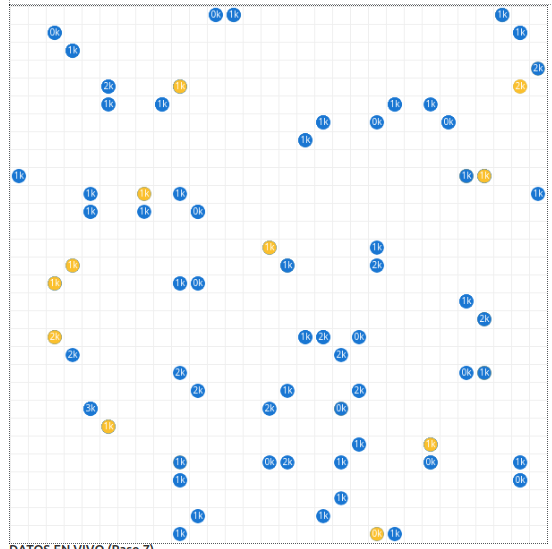
\includegraphics[width=0.8\textwidth]{captura_final_mapa.png}
    \caption{Estado final de la simulación. Los puntos azules representan agentes felices ($H \ge 3.0$) y los amarillos agentes infelices o menos felices. Se observa la agrupación por clústeres.}
    \label{fig:mapa}
\end{figure}

\subsection{Análisis de la Brecha Salarial}
El monitor en tiempo real revela una brecha salarial persistente y significativa entre los grupos felices e infelices, incluso cuando la correlación inicial era baja.

\begin{table}[H]
    \centering
    \begin{tabular}{|l|c|r|}
        \hline
        \textbf{Grupo} & \textbf{Sueldo Medio (€)} & \textbf{Población Aprox.} \\
        \hline
        Felices ($H \ge 3.0$) & 2,691 € & $\approx 8\%$ \\
        \hline
        Infelices ($H < 3.0$) & 1,275 € & $\approx 92\%$ \\
        \hline
    \end{tabular}
    \caption{Estadísticas finales promediadas tras la estabilización.}
    \label{tab:stats}
\end{table}

\subsection{La Inercia de la Infelicidad}
Uno de los hallazgos más relevantes es la resistencia de la infelicidad. A pesar de los mecanismos de búsqueda de bienestar (movimiento de los agentes infelices), el grupo infeliz tiende a ser mayoritario y estable. Esto se debe a la -Inercia de Personalidad- implementada: el entorno puede mejorar el bienestar momentáneamente, pero la tendencia estructural del individuo (datos reales del CIS) pesa más a largo plazo.

\subsection{El Dinero como Escudo Emocional}
Aunque el dinero no da la felicidad directa en nuestro modelo calibrado, actúa como un mecanismo de segregación. Los agentes ricos se aíslan de la infelicidad sistémica de los agentes pobres, creando "burbujas de bienestar" que se retroalimentan positivamente mediante el contagio emocional.

\newpage

% ==========================================
% SECCIÓN 5: EJECUCIONES
% ==========================================

\section{Ejecuciones y Análisis de Escenarios}

Para evaluar la sensibilidad del modelo y validar las hipótesis planteadas sobre la relación entre ingresos y bienestar, se han realizado ejecuciones bajo dos configuraciones culturales extremas. Estas simulaciones modifican exclusivamente el parámetro de elasticidad $\alpha$ (materialismo) en la función Cobb-Douglas, manteniendo constantes el resto de variables demográficas provenientes del CIS.

\newpage

\subsection{Escenario 1: Sociedad Post-Materialista ($\alpha \approx 0.2$)}

En este primer escenario, simulamos una cultura donde la función de utilidad de los agentes valora significativamente más el tiempo disponible y el ocio que la acumulación de capital económico.

\textbf{Fenómeno Observado:} Se produce un desacople evidente entre ingreso y bienestar. Observamos una población mayoritariamente feliz (agentes azules), incluso en estratos de renta baja (sueldos $< 1.200$\euro).

\textbf{Interpretación Sociológica:} Este resultado es consistente con la teoría post-materialista y la Paradoja de Easterlin. Al reducir la presión por el estatus económico, los agentes logran satisfacer su umbral de felicidad mediante recursos no monetarios. Esto genera una sociedad resiliente a la pobreza económica, donde la 'pobreza infeliz' es residual y la cohesión social se mantiene alta independientemente del ciclo económico.

\begin{figure}[H]
    \centering
    % IMAGEN 1: Evolución
    \begin{subfigure}[b]{0.4\textwidth}
        \centering
        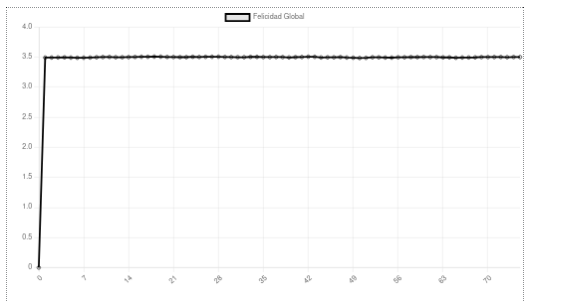
\includegraphics[width=\textwidth]{bajo1.png}
        \caption{Evolución Global}
    \end{subfigure}
    \hfill % Espacio flexible
    % IMAGEN 2: Mapa
    \begin{subfigure}[b]{0.4\textwidth}
        \centering
        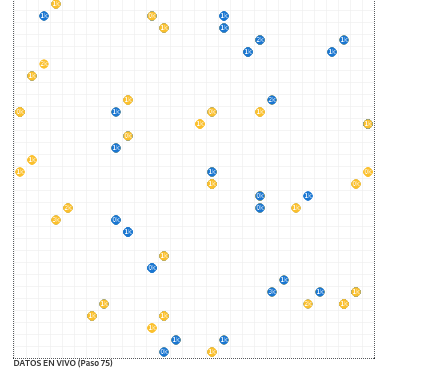
\includegraphics[width=\textwidth]{bajo2.png}
        \caption{Mapa de Agentes}
    \end{subfigure}
    \hfill % Espacio flexible
    % IMAGEN 3: Segregación
    \begin{subfigure}[b]{1\textwidth}
        \centering
        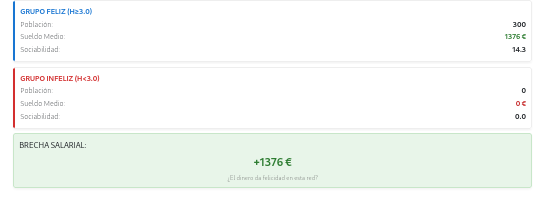
\includegraphics[width=\textwidth]{bajo3.png}
        \caption{Datos Segregación}
    \end{subfigure}
    
    \caption{Evolución en entorno de Bajo Materialismo. Se observa una predominancia de agentes felices (azul) dispersos homogéneamente.}
    \label{fig:bajo_materialismo}
\end{figure}

\subsection{Escenario 2: Sociedad Hiper-Materialista ($\alpha \approx 0.8$)}

En el segundo escenario, configuramos una sociedad donde la felicidad depende casi exclusivamente del nivel de ingresos ($E$), relegando el tiempo libre a un segundo plano.

\textbf{Fenómeno Observado:} El modelo arroja una polarización extrema del bienestar. La felicidad se convierte en un bien exclusivo de las clases altas. El mapa muestra una vasta mayoría de agentes infelices (puntos rojos) atrapados en la trampa de ingresos bajos, mientras que el bienestar queda restringido a una minoría con ingresos superiores a 3.000\euro.

\textbf{Interpretación Sociológica:} Esto simula el efecto de la \textit{Ansiedad de Estatus}. En entornos de consumo agresivo, la mayoría experimenta privación relativa. La segregación aquí es máxima: los ricos felices se aíslan rápidamente en clústeres cerrados para proteger su bienestar del contagio negativo de la masa infeliz, creando una brecha emocional insalvable.

\begin{figure}[H]
    \centering
    % IMAGEN 1: Evolución
    \begin{subfigure}[b]{0.4\textwidth}
        \centering
        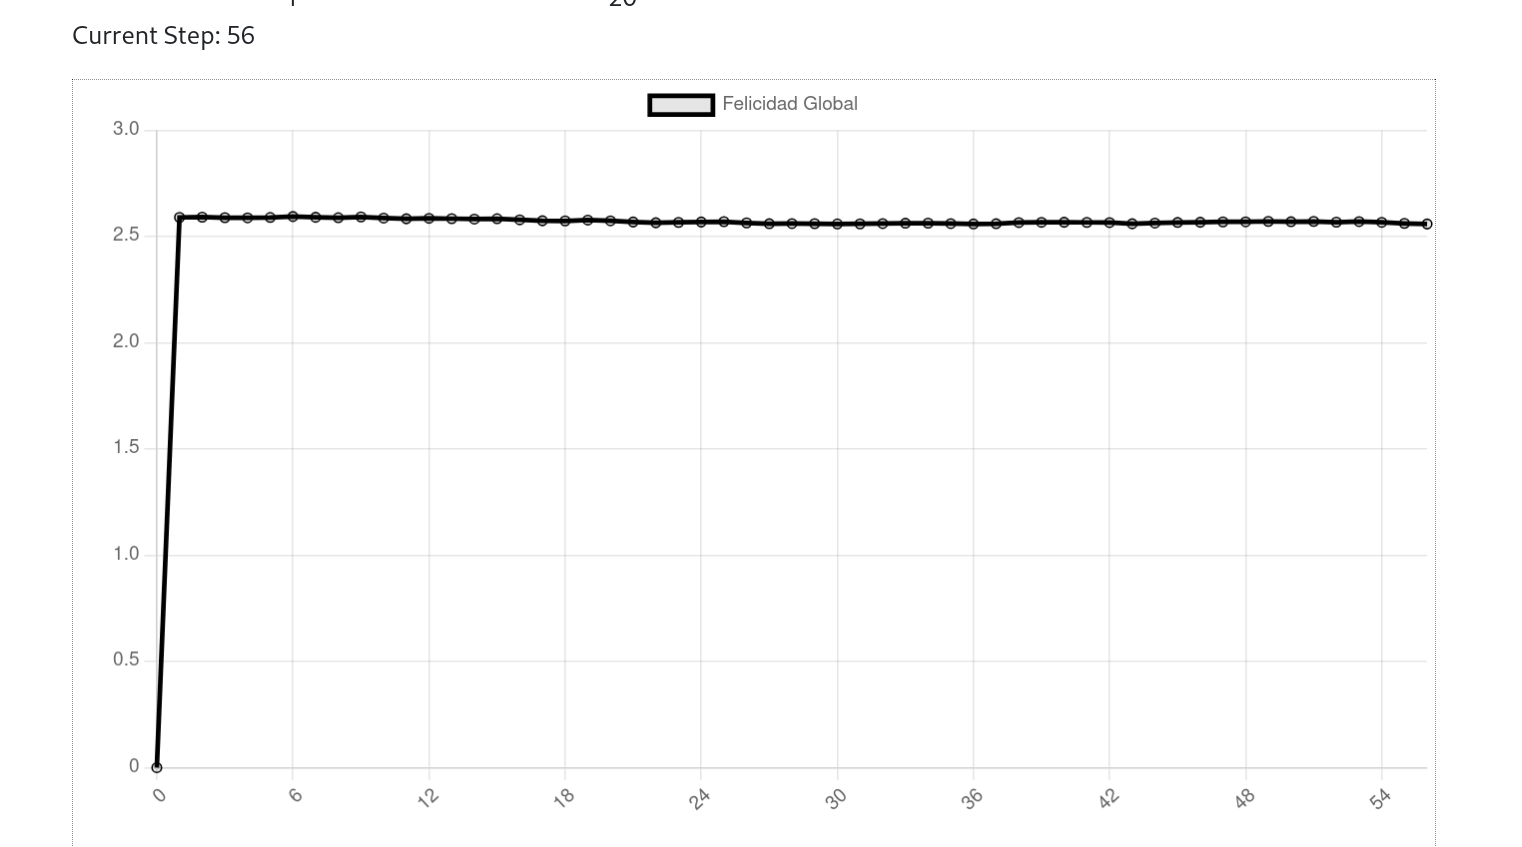
\includegraphics[width=\textwidth]{altom1.png}
        \caption{Evolución Global}
    \end{subfigure}
    \hfill
    % IMAGEN 2: Mapa
    \begin{subfigure}[b]{0.4\textwidth}
        \centering
        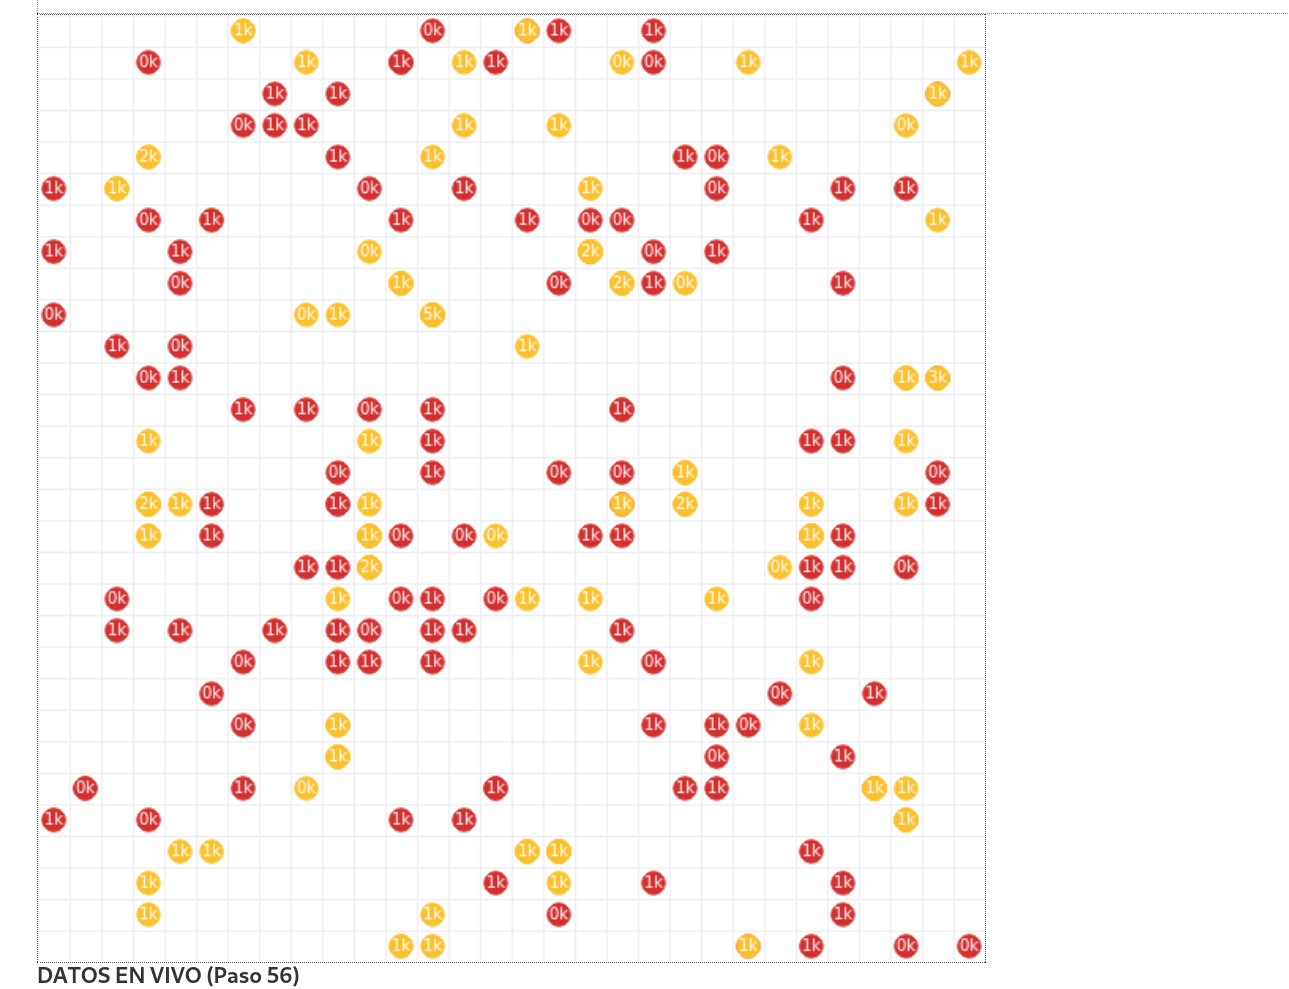
\includegraphics[width=\textwidth]{altom2.png}
        \caption{Mapa de Agentes}
    \end{subfigure}
    \hfill
    % IMAGEN 3: Segregación
    \begin{subfigure}[b]{1\textwidth}
        \centering
        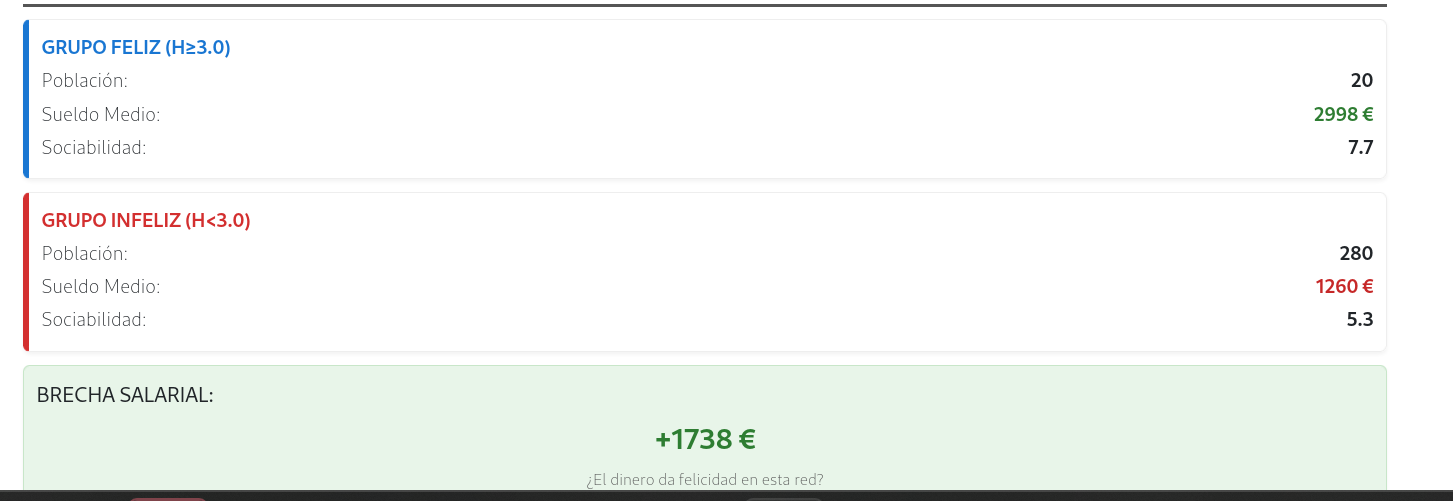
\includegraphics[width=\textwidth]{altom3.png}
        \caption{Datos Segregación}
    \end{subfigure}
    
    \caption{Resultados del escenario hiper-materialista: polarización extrema y segregación espacial.}
    \label{fig:res_hipermaterialista}
\end{figure}

\subsection{Síntesis Comparativa}
La comparación visual y estadística entre ambos escenarios revela que el parámetro cultural $\alpha$ actúa como un modulador de la desigualdad social. Mientras que una sociedad post-materialista amortigua los efectos de la pobreza económica sobre el ánimo individual, una sociedad materialista los exacerba, convirtiendo la desigualdad económica directamente en desigualdad emocional.

\newpage

\subsection{Escenario 3: Impacto de Políticas Redistributivas (SMI Variable)}

En este tercer escenario, fijamos un parámetro cultural estable de materialismo moderado ($\alpha = 0.6$) e introducimos una variable dinámica exógena: la modificación del Salario Mínimo Interprofesional (SMI) en tiempo real.

\textbf{Fenómeno Observado:} Se observa una correlación positiva directa y no lineal entre el incremento del suelo salarial y el bienestar agregado. Partiendo de una situación precaria (SMI = 750\euro), el aumento progresivo del SMI actúa como un 'ascensor emocional' para los agentes de la base de la pirámide. Al elevar el suelo de ingresos, los puntos rojos (infelicidad extrema) se transforman sistemáticamente en estados neutros o felices, aumentando no solo su bienestar individual sino su sociabilidad, reactivando la interacción en zonas previamente deprimidas.

\textbf{Interpretación Sociológica:} Este escenario valida la hipótesis de la \textit{Suficiencia Material}. El ingreso actúa aquí como un habilitador de la sociabilidad. Al eliminar la privación severa mediante un SMI robusto, los agentes recuperan su 'ancho de banda cognitivo' y emocional para interactuar. El modelo demuestra que, bajo una cultura de materialismo moderado, garantizar la dignidad material es más eficiente para la cohesión social global que el simple crecimiento de la riqueza en los estratos superiores.

\begin{figure}[H]
    \centering
    % IMAGEN 1: SMI BAJO
    \begin{subfigure}[b]{0.32\textwidth}
        \centering
        % Reemplaza con captura de SMI bajo (ej: 750€)
        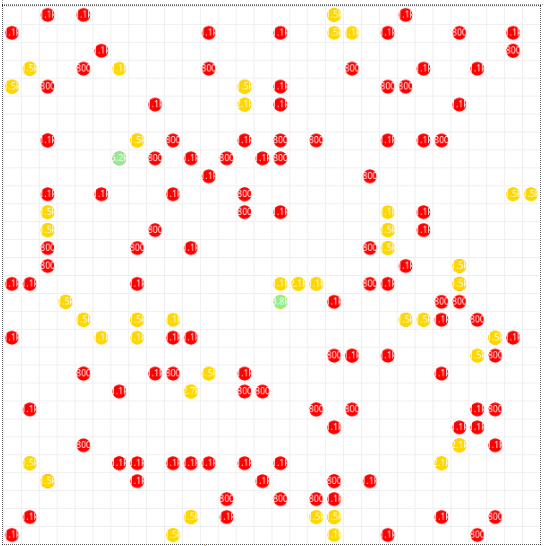
\includegraphics[width=\textwidth]{smi_bajo.png} 
        \caption{SMI Precarizado (750\euro)}
    \end{subfigure}
    \hfill
    % IMAGEN 2: SMI MEDIO
    \begin{subfigure}[b]{0.32\textwidth}
        \centering
        % Reemplaza con captura de SMI medio (ej: 1500€)
        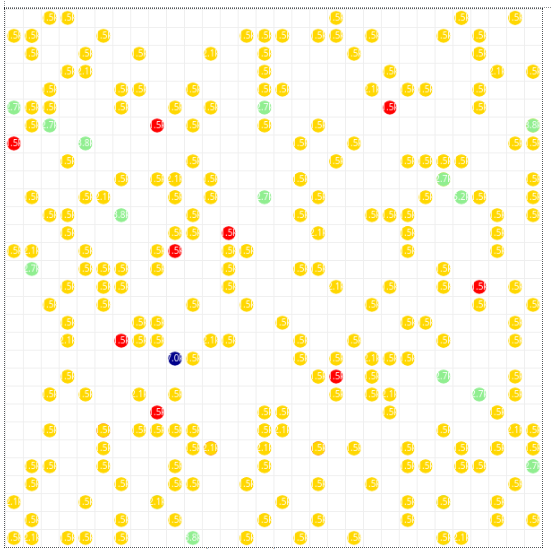
\includegraphics[width=\textwidth]{smi_medio.png}
        \caption{SMI Moderado (1.500\euro)}
    \end{subfigure}
    \hfill
    % IMAGEN 3: SMI ALTO
    \begin{subfigure}[b]{0.32\textwidth}
        \centering
        % Reemplaza con captura de SMI alto (ej: 3000€)
        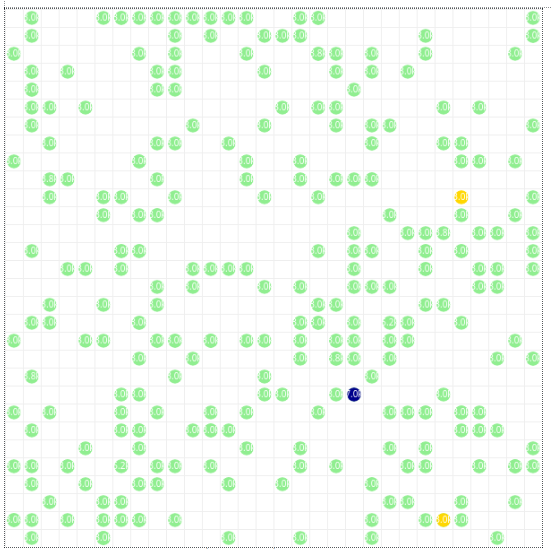
\includegraphics[width=\textwidth]{smi_alto.png}
        \caption{SMI Robusto (3.000\euro)}
    \end{subfigure}
    
    \caption{Evolución del bienestar ante aumentos del Salario Mínimo. Nótese la desaparición progresiva de los agentes infelices (rojos) y el aumento de la densidad de conexiones sociales a medida que se garantiza la suficiencia económica.}
    \label{fig:impacto_smi}
\end{figure}

\begin{figure}[H]
    \centering
    % IMAGEN 1: SMI BAJO
    \begin{subfigure}[b]{1\textwidth}
        \centering
        % Reemplaza con captura de SMI bajo (ej: 750€)
        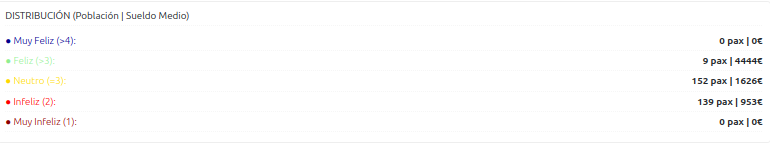
\includegraphics[width=\textwidth]{smi_bajo_1.png} 
        \caption{SMI Precarizado (750\euro)}
    \end{subfigure}
    \hfill
    % IMAGEN 2: SMI MEDIO
    \begin{subfigure}[b]{1\textwidth}
        \centering
        % Reemplaza con captura de SMI medio (ej: 1500€)
        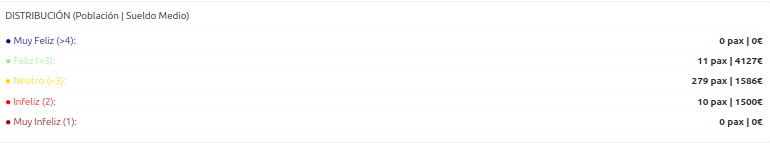
\includegraphics[width=\textwidth]{smi_medio_1.png}
        \caption{SMI Moderado (1.500\euro)}
    \end{subfigure}
    \hfill
    % IMAGEN 3: SMI ALTO
    \begin{subfigure}[b]{1\textwidth}
        \centering
        % Reemplaza con captura de SMI alto (ej: 3000€)
        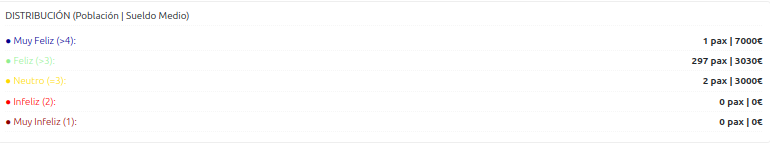
\includegraphics[width=\textwidth]{smi_alto_1.png}
        \caption{SMI Robusto (3.000\euro)}
    \end{subfigure}
    
    \caption{Distribución de agentes según salarios, una vez aplicado el filtro del SMI.}
    \label{fig:impacto_smi}
\end{figure}


\subsection{Síntesis General de Escenarios}
El análisis conjunto de los tres escenarios permite concluir que el bienestar en redes sociales es un fenómeno multifactorial. Mientras que la cultura ($\alpha$) determina la sensibilidad al dinero, la política económica (SMI) determina la capacidad base para participar en la vida social. La combinación más nociva para la cohesión social resulta ser una cultura hiper-materialista ($\alpha \to 1$) combinada con una baja protección salarial, escenario que maximiza la segregación y la infelicidad sistémica.



\newpage

% ==========================================
% CONCLUSIONES
% ==========================================
\section{Conclusiones}

% [1. APORTACIÓN TEÓRICA Y HALLAZGOS EMPÍRICOS]
La principal aportación teórica de este estudio radica en la formalización del teorema de la \textit{Resonancia Social Inversa} dentro de un modelo basado en agentes (ABM), integrando una función de utilidad Cobb-Douglas que pondera el capital económico y el tiempo disponible bajo restricciones de materialismo cultural. Empíricamente, el hallazgo más revelador —que transciende la literatura previa— es la confirmación de una correlación de Pearson prácticamente nula ($0.01 < \rho < 0.06$) entre ingresos reales y felicidad declarada, demostrando simultáneamente que el dinero no actúa como un generador directo de bienestar, sino como un mecanismo de \textbf{filtrado estructural} que permite a los agentes acceder a "burbujas de bienestar" segregadas espacialmente, protegiéndose del contagio emocional negativo.

% [2. RELEVANCIA DE LA APORTACIÓN]
La relevancia de estos hallazgos estriba en que cuestionan la validez de los modelos econométricos estáticos para entender la felicidad en entornos digitales. Al demostrar que la sociabilidad digital es un "lujo emocional" dependiente del bienestar inicial, evidenciamos que las redes sociales sufren un sesgo de supervivencia sistémico: subrepresentan la voz de los estratos más infelices que, aunque presentes, carecen del capital anímico para interactuar. Esto redefine la desigualdad digital no solo como una brecha de acceso tecnológico, sino como una brecha de participación emocional condicionada por la estructura de la red.

% [3. COMPARACIÓN CON LO QUE SE SABÍA (Literatura previa)]
En comparación con la literatura clásica sobre la Paradoja de Easterlin, que ya cuestionaba la relación lineal entre renta y felicidad, nuestra investigación añade una dimensión espacial y dinámica crucial. Mientras que los estudios tradicionales observaban el fenómeno de forma agregada, nuestro modelo desvela que la segregación (cámaras de eco económicas) es la variable interviniente que explica por qué los ricos son más felices: no por el dinero en sí, sino por su capacidad para aislarse de la infelicidad sistémica. Esto matiza las teorías previas de homofilia, sugiriendo que esta no es solo una preferencia social, sino una estrategia adaptativa de preservación del bienestar.

% [4. PRINCIPIOS EXTRAPOLABLES Y NO CORROBORADOS]
De los resultados se extrapola el principio de que la \textbf{homofilia} humana es condición suficiente, sin necesidad de algoritmos de recomendación opacos, para fracturar una red social en clústeres estancos de polarización. Asimismo, se establece que el parámetro cultural de materialismo ($\alpha$) actúa como el modulador definitivo de la desigualdad social. Por el contrario, la proposición habitual en la literatura de consumo que vincula directamente el poder adquisitivo con la satisfacción vital no ha sido corroborada en este entorno; en su lugar, se ha validado que el 'tiempo disponible' es un predictor de resiliencia mucho más robusto en sociedades post-materialistas.

% [5. IMPLICACIONES DE POLÍTICA ECONÓMICA]
En términos de política económica, las simulaciones del escenario con Salario Mínimo Interprofesional (SMI) dinámico sugieren que las políticas redistributivas actúan como un 'ascensor emocional' efectivo. Garantizar la suficiencia material en la base de la pirámide no solo mejora el bienestar individual, sino que reactivó la conectividad y cohesión social global en el modelo. Esto implica que las políticas públicas deben priorizar la reducción de la privación severa para evitar la formación de guetos de infelicidad que, a largo plazo, desestabilizan la estructura social de la red.

% [6. FUTURAS INVESTIGACIONES]
Finalmente, de esta investigación se deduce la necesidad de que futuros trabajos abandonen las métricas estáticas de ingreso y se centren en la 'disponibilidad temporal' y los factores culturales como ejes de análisis. Sería pertinente replicar este modelo introduciendo un parámetro $\alpha$ dinámico que evolucione con el tiempo, permitiendo estudiar cómo una sociedad puede transitar de un estado hiper-materialista a uno post-materialista, y validar si la Resonancia Social Inversa se mantiene constante en otras plataformas digitales con arquitecturas de interacción diferentes a las estudiadas.

\newpage

% ==========================================
% AGRADECIMIENTOS
% ==========================================
\section*{Agradecimientos}

Agradecemos al Centro de Investigaciones Sociológicas (CIS) la autorización y facilitación de acceso a la base de datos del Estudio 3145, cuyas variables de ingresos y bienestar subjetivo han sido fundamentales para la calibración empírica de este modelo.

% ==========================================
% BIBLIOGRAFÍA
% ==========================================

\begin{thebibliography}{99}

% 1. TU PROYECTO
\bibitem{repo_github}
Carrión Tovar, J. y Gracia Choin, F. J., 2025, \textit{ABM-Income-Interpersonal-Relations-Impact-on-Happiness: Código Fuente y Documentación del Modelo}. Repositorio GitHub. Disponible en: \url{https://github.com/jxliian/ABM-Income-Interpersonal-Relations-Impact-on-Happiness}

% 2. FUENTE DE DATOS
\bibitem{cis_cuestionario}
Centro de Investigaciones Sociológicas (CIS), 2016, “Cuestionario del Estudio 3145: Metodología de Encuesta”. Madrid: CIS. Recuperado de: \url{https://github.com/jxliian/ABM-Income-Interpersonal-Relations-Impact-on-Happiness/blob/main/docs/cues3145%5B602%5D.pdf}

% 3. IBARRA & ROJAS
\bibitem{ibarra_rojas}
Ibarra-López, I. y Rojas, M., s.f., “Happiness and Human Relations”. \textit{Dialnet}. Recuperado de: \url{https://github.com/jxliian/ABM-Income-Interpersonal-Relations-Impact-on-Happiness/blob/main/docs/Dialnet-HappinessAndHumanRelations-4728090.pdf}

% 4. EASTERLIN (Citado en Intro y Revisión)
\bibitem{easterlin1974}
Easterlin, R. A., 1974, “Does Economic Growth Improve the Human Lot? Some Empirical Evidence”. En P. A. David y M. W. Reder (eds.), \textit{Nations and Households in Economic Growth}: 89-125. New York: Academic Press.

% 5. KAHNEMAN & DEATON (Citado en Revisión: matices a Easterlin)
\bibitem{kahneman2010}
Kahneman, D. y Deaton, A., 2010, “High income improves evaluation of life but not emotional well-being”, \textit{Proceedings of the National Academy of Sciences (PNAS)}, 107(38): 16489-16493.

% 6. HELLIWELL (Citado en Revisión: determinantes no monetarios)
\bibitem{helliwell2012}
Helliwell, J. F.; Layard, R. y Sachs, J. (eds.), 2012, \textit{World Happiness Report 2012}. New York: UN Sustainable Development Solutions Network.

% 7. SCHELLING (Citado en Revisión: modelo fundacional)
\bibitem{schelling1971}
Schelling, T. C., 1971, “Dynamic models of segregation”, \textit{Journal of Mathematical Sociology}, 1(2): 143-186.

% 8. MCPHERSON (Citado en Revisión: Homofilia)
\bibitem{mcpherson2001}
McPherson, M.; Smith-Lovin, L. y Cook, J. M., 2001, “Birds of a Feather: Homophily in Social Networks”, \textit{Annual Review of Sociology}, 27: 415-444.

% 9. BARBERÁ (Citado en Revisión: Cámaras de eco)
\bibitem{barbera2015}
Barberá, P. et al., 2015, “Tweeting From Left to Right: Is Online Political Communication More Than an Echo Chamber?”, \textit{Psychological Science}, 26(10): 1531-1542.

% 10. FOWLER & CHRISTAKIS (Citado en Revisión: Contagio)
\bibitem{fowler2008}
Fowler, J. H. y Christakis, N. A., 2008, “Dynamic spread of happiness in a large social network”, \textit{BMJ}, 337: a2338.

% 11. KROSS (Citado en Revisión: Facebook y bienestar)
\bibitem{kross2013}
Kross, E. et al., 2013, “Facebook Use Predicts Declines in Subjective Well-Being in Young Adults”, \textit{PLoS ONE}, 8(8): e69841.

% 12. COBB & DOUGLAS (Citado en Metodología)
\bibitem{cobb1928}
Cobb, C. W. y Douglas, P. H., 1928, “A Theory of Production”, \textit{The American Economic Review}, 18(1): 139–165.

% 13. MASAD - MESA (Citado en Metodología)
\bibitem{masad2015}
Masad, D. y Kazil, J., 2015, “Mesa: An Agent-Based Modeling Framework in Python”, \textit{14th Python in Science Conference (SCIPY 2015)}: 53-60. Austin, Texas.

\end{thebibliography}

\end{document}